% standard LaTeX packages
\documentclass[11pt,a4paper]{article}

\usepackage[utf8]{inputenc}
\usepackage[T1]{fontenc}
\usepackage[english]{babel}
\usepackage[margin=3cm]{geometry}
\usepackage{parskip}
\usepackage{xifthen}
\usepackage{placeins} %Floatbarrier
\usepackage{graphicx} %package to manage images
\usepackage{subcaption}

% math packages
\usepackage{mathtools,amsfonts,amssymb,mathdots}
\usepackage{siunitx}

\usepackage[rightcaption]{sidecap}

\newcommand{\dd}[1]{\mathrm{d}#1} %numbering
% plotting and tables
\usepackage{tikz}
\usepackage{pgfplots}
\usepackage{pgfplotstable}
\usepackage{caption}
% other packages
\usepackage{filecontents}


\begin{document}

\title{Prosjekt 3: Modell av solsystemet ved hjelp av ordinære differensialligninger }
\author{Live Wang Jensen (\texttt{livewj}) \\ Joseph Knutson (\texttt{josephkn})}
\date{\today}

\maketitle

\begin{abstract}
skfjsk
\end{abstract}

\tableofcontents

\clearpage
\section{Introduksjon}
Målet med dette prosjektet er å utvikle en kode som kan simulere solsystemet ved hjelp av den populære \textit{velocity Verlet} algoritmen. I første del skal vi se på et forenklet solsystem med Jorden som eneste planet kretsende rundt Solen. Dette gjøres for å teste selve algoritmen og se om alt fungerer. Her skal vi teste både Eulers metode og velocity Verlet metoden, men videre skal vi kun bruke Verlet metoden, da denne er mye mer stabil. Den eneste kraften som virker i systemet vårt er tyngdekraften. Vi innfører deretter Jupiter og observerer hvordan Jupiters masse vil påvirke Jordens bane omkring Solen. Til slutt skal vi modellere et fullstendig solsystem med alle planeter, og se på hvordan dette oppfører seg som funksjon av tiden. I tillegg skal vi se spesielt på Merkurs bane og hvordan den påvirkes av den relativistiske tyngdekraften. SKRIV MER HER

\section{Teori}
Det er kun tyngdekraften som virker på systemet vårt. Newtons tyngdelov sier at tyngdekraften som virker mellom to legemer, er proporsjonal med produktet av deres masse, og omvendt proporsjonal med kvadratet av avstanden mellom dem [5]. Dersom vi skal se på tyngdekraften som virker mellom Solen og Jorden, kan loven kan uttykkes på følgende måte:
\begin{equation}
F_G = \frac{GM_{\odot}M_{Earth}}{r^2}
\end{equation}
hvor $M_{\odot}$ er Solens masse, $M_{Earth}$ er Jordens masse, $G$ er gravitasjonskonstanten og $r$ er avstanden mellom Jorden og Solen. Vi antar at massen til Solen er mye større enn massen til Jorden, slik at vi kan se bort fra tyngdekraften som virker på Solen i Jord-Sol-systemet. \\

Dersom vi antar at Jordens bane rundt Solen ligger i $xy$-planet, kan vi bruke Newtons andre lov til å finne
\begin{equation}
 \frac{d^2x}{dt^2}=\frac{F_{G,x}}{M_{\mathrm{Earth}}}
\end{equation}
og 
\begin{equation}
\frac{d^2y}{dt^2}=\frac{F_{G,y}}{M_{\mathrm{Earth}}}
\end{equation}

hvor $F_{G,x}$ og $F_{G,y}$ er $x$ og $y$ komponentene til tyngdekraften. I dette prosjektet skal vi bruke astronomiske enheter (AU). Èn astronomisk enhet er altså den gjennomsnittlige avstanden mellom Jorden og Solen, 1 AU = 1.5$\times10^{11}$m. I tillegg bruker vi enheten år i stedet for sekunder til å måle tiden med. I vårt system er Solens masse skalert slik at $M_{\odot} = 1$. Massen til alle de andre planetene skaleres derfor i forhold til solmassen, for eksempel vil $M_{Earth,skalert} = M_{\odot}/M_{Earth}$. 


\section{Løsningsmetoder}
Vi kan beregne Jordens bane rundt Solen ved å bruke enten Eulers metode eller velocity Verlet algoritmen til å løse de ordinære differensialligningene gitt ovenfor. Dersom vi antar at Jorden beveger seg i en sirkulær bane rundt Solen, vet vi i følge Newtons andre lov at tyngkraften som virker på Jorden må være
\[F_G = \frac{M_{Earth}v^2}{r} = \frac{GM_{\odot}M_{Earth}}{r^2}  \]
siden $a = v^2/r$ for en sirkulær bane, hvor $v$ er Jordens hastighet. Denne ligningen kan brukes til å vise at 
\[v^2r = GM_{\odot} = 4\pi^2 AU^3/yr^2  \]

\subsection{Euler}
Vi kan diskretisere ligningene gitt ovenfor slik at vi kan sette opp en algoritme for å løse ligningene ved hjelp av Eulers metode. Dersom vi har en funksjon $y$, kan vi finne ut hvordan funksjonen ser ut i et tidssteg $y_{i+1}$ ved hjelp av det tidligere tidssteget $y_i$:
\[y_{i+1} = y(t= t_i + h) = y(t_i) + h\Delta(t_i, y_i(t_i)) + O(h^{p+1}) \]
hvor $h = (b - a)/N$ er steglengden, $N$ er antall tidssteg, $a$ og $b$ er integrasjonsgrensen og $O(h^{p+1})$ er feilen i beregningen vår. $\Delta$ representerer alle de deriverte av funksjonen vår $y$:
\[\Delta(t_i, y_i(t_i)) = (y'(t_i) + ... + y^{(p)}(t_i)\frac{h^{p-1}}{p!} )  \]
Hvis vi definerer
\[y'(t_i) = f(t_i, y_i) \]
og minker $\Delta$ til å kun inneholde den førstederiverte av $y$, får vi
\[y_{i+1} = y(t_i) + hf(t_i,y_i) + O(h^2)  \]
og 
\[t_{i+1} = t_i + h \]
som sammen utgjør Eulers metode. Legg merke til at vi for hvert tidssteg får en feil på $O(h^2)$. Dette gir oss en global feil på $N\cdot O(h^2) \approx O(h)$  [7]. Eulers metode er altså ikke å anbefale hvis vi ønsker nøyaktighet i beregningene, men kan være nyttig dersom vi ønsker et førsteintrykk av hvordan løsningen kan se ut. \\

Et eksempel på hvordan dette kan implementeres i C++ vises i figur \ref{euler}. Her er \texttt{Euler} en funksjon i klassen med samme navn. Funksjonen starter med å hente funksjonen \texttt{calculateForcesAndEnergy()} fra klassen vår \texttt{SolarSystem}, som inneholder alle de nødvendige metodene for å simulere solsystemet, bortsett fra integrasjonsmetodene. Inne i for-løkken beregnes legemenes posisjon og hastighet ved hjelp av Eulers algoritme.

\FloatBarrier
\begin{figure}[!ht]
\begin{center}
  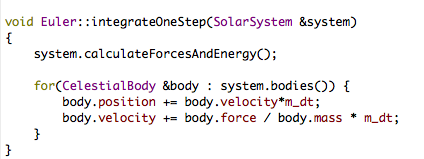
\includegraphics[width = 100mm]{euler.png}\\
  \caption{Eksempel på hvordan Eulers algoritme kan implementeres i en klasse i C++. Koden er hentet fra filen \texttt{euler.cpp}.}   \label{euler}
  \end{center}
  \end{figure}
\FloatBarrier


\subsection{Velocity Verlet}
En annen metode å løse differensialligningene på er Verlet metoden. Denne populære algoritmen er både numerisk stabil og enkel å implementere. Dersom vi tar for oss Newtons andre lov som en andre ordens differensialligning, som i én dimensjon kommer på formen
\[ m \frac{d^2x}{dt^2} = F(x,t) \]
som kan skrives om til to \textit{koblede} differensialligninger
\[\frac{dx}{dt} = v(x,t) \quad og \quad \frac{dv}{dt} = F(x,t)/m = a(x,t) \]
Dersom vi nå gjør en Tayorutvikling
\begin{equation}
x(t+h) = x(t) + hx^{(1)}(t) + \frac{h^2}{2}x^{(2)}(t) + O(h^3)
\label{1}
\end{equation}
I vårt tilfelle kjenner vi den andrederiverte via Newtons andre lov, $x^{(2)} = a(x,t)$. Dersom vi legger til Taylorutviklingen for $x(t-h)$ i ligning \ref{1}, ender vi opp med 
\[x_{i+1} = 2x_i - x_{i-1} + h^2x_i^{(2)} + O(h^4) \]
hvor $x_{i\pm 1} = x(t_i \pm h)$ og $x_i = x(t_i)$. Feilen her går som $O(h^4)$, siden alle de odde leddene kansellerer i addisjonen [7]. Hastigheten er ikke direkte inkludert i ligningen, siden $x^{(2)}$ er kjent. Dersom vi trenger hastigheten, kan vi finne den ved å bruke ligningen
\[x_i^{(1)} = \frac{x_{i+1} - x_{i+1}}{2h} + O(h^2) \]
Hastigheten har altså en feil på $O(h^2)$. Legg merke til at algoritmen for posisjonen $x$ for $i=0$ trenger den ikke-eksisterende verdien $x_{-1}$ for å starte. Dette problemet unngås i \textbf{velocity Verlet} metoden. Taylorutviklingen til posisjonen er gitt som
\[x_{i+1} = x_i + hx_i^{(1)} + \frac{h^2}{2}x_i^{(2)} + O(h^3) \]
mens Taylorutviklingen til hastigheten er 
\[v_{i+1} = v_i + hv_i^{(1)} + \frac{h^2}{2}v_i^{2} + O(h^3) \]
Ved hjelp av Newtons andre lov har vi et analytisk uttrykk for den deriverte til hastigheten, nemlig
\[ v_i^{(1)} = \frac{d^2x}{dt^2}|_i = \frac{F(x_i, t_i)}{m} \]

Dersom vi adderer dette til Taylorutviklingen til akselerasjonen
\[v_{i+1}^{(1)} = v_i^{(1)} + hv_i^{(2)} + O(h^2) \]
og ser bort fra de høyere ordens leddene etter den andrederiverte av hastigheten, får vi 
\[hv_i^{(2)} \approx v_{i+1}^{(1)} - v_i^{(1)}  \]
Vi kan nå skrive om Taylorutviklingen til hastigheten som
\[ v_{i+1} = v_i + \frac{h}{2}\left( v_{i+1}^{(1)} + v_i^{(1)} \right) + O(h^3)  \]

Det vi ender opp med til slutt er den berømte \textbf{velocity Verlet} algoritmen:
\[x_{i+1} = x_i + hv_i + \frac{h^2}{2}v_i^{(1)} + O(h^3)  \]
\[v_{i+1} = v_i + \frac{h}{2} \left( v_{i+1}^{(1)} + v_i^{(1)} \right) + O(h^3)  \]

Implementasjonen finnes i filen \texttt{velocityverlet.cpp}, og et lite utsnitt av denne algortimen vises i figur \ref{vv}. Funksjonen \texttt{VelocityVerlet} starter med å initialisere kreftene som virker på systemet ved hjelp av funksjonen \texttt{calculateForcesAndEnergy}, før den bruker velocity Verlet metoden til å beregne legmenes hastighet og posisjon. Etter at dette er gjort, oppdateres kreftene før hastigheten beregnes igjen.

\FloatBarrier
\begin{figure}[!ht]
\begin{center}
  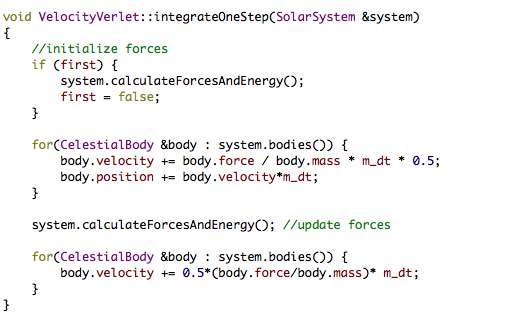
\includegraphics[width = 100mm]{vv.png}\\
  \caption{Eksempel på hvordan velocity Verlet algoritmen kan implementeres i en klasse i C++. Koden er hentet fra filen \texttt{velocityverlet.cpp}.}   \label{vv}
  \end{center}
  \end{figure}
\FloatBarrier

\section{Resultater}
\subsection{Unnslipningshastighet}
Ved hjelp av prøving og feiling, fant vi unnslipningshastigheten til Jorden i en avstand 1 AU fra Solen. Dette ble gjort ved å sette jordens posisjon lik $(1,0,0)$ og hastighet $(0,v_y,0)$. Ved å variere verdien til $v_y$ fant vi at unnslipningshastigheten må ligge et sted mellom $v_y$ = 8.75 og $v_y$ = 8.90, se figur \ref{fig:uh}. 

\FloatBarrier
\begin{figure}[!ht]
\centering
\begin{subfigure}{.5\textwidth}
  \centering
  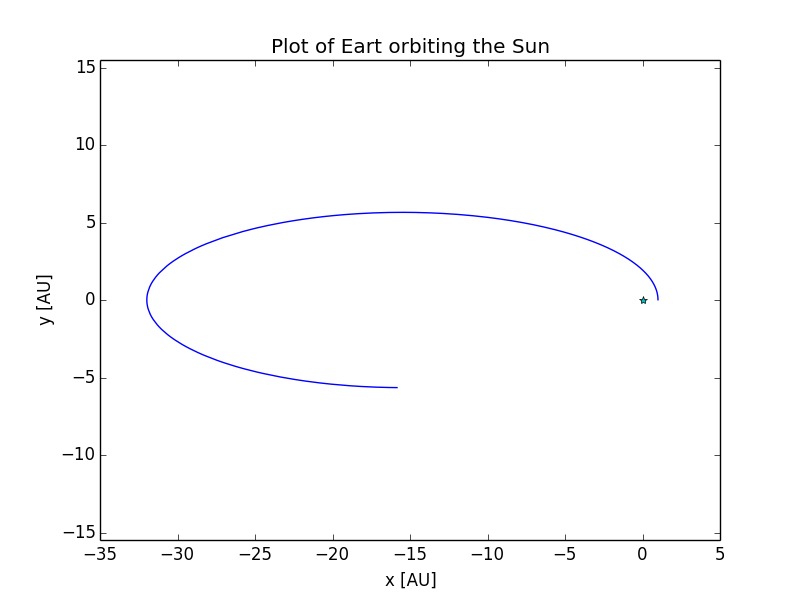
\includegraphics[width=1.1\linewidth]{3d_escape_v_8_75.png}
  \caption{$v_y$ = 8.75}
  \label{fig:sub1}
\end{subfigure}%
\begin{subfigure}{.5\textwidth}
  \centering
  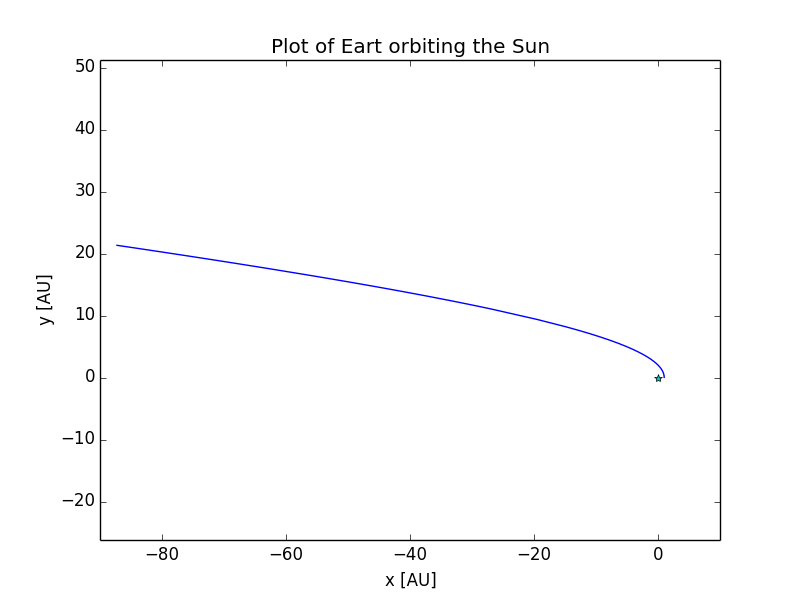
\includegraphics[width=1.1\linewidth]{3d_escape_v_8_9.png}
  \caption{$v_y$ = 8.90}
  \label{fig:sub2}
\end{subfigure}
\caption{Figurene viser Jordens bane for ulike unnslipningshastigheter. Vi ser at denne hastigheten må ligge et sted mellom 8.75 og 8.90. I dette tilfellet er det ingen krefter som virker på Solen, og den er markert med en stjerne i origo.}
\label{fig:uh}
\end{figure}
\FloatBarrier

Vi kan finne et eksakt svar ved hjelp av Newtons andre lov:
\[F = m\cdot a = m \cdot\frac{v^2}{r} \]
hvor vi har brukt at akselerasjonen i en sirkulær bane er $a=v^2/r$. Her er $v$ Jordens hastighet og $r$ avstanden mellom Solen og Jorden, som i dette tilfellet er 1 AU. Den eneste kraften som virker på jorden er tyngdekraften, slik at
\[G \frac{M_{\odot}M_{Earth}}{r^2} = \frac{v^2}{r} \]
Massen til Solen er $M_{\odot}$ = 1, og vi ender opp med
\[\sqrt{GM_{Earth}} = v  \]
\[\sqrt{4\pi^2}  \]



\subsection{Test av algoritmen}

\section{Diskusjon}
\section{Konklusjon}



=== Project 3a): The Earth-Sun system 

We assume that mass units can be obtained by using the fact that Earth's orbit is almost circular around the Sun.
For circular motion we know that the force must obey the following relation
\[
F_G= \frac{M_{\mathrm{Earth}}v^2}{r}=\frac{GM_{\odot}M_{\mathrm{Earth}}}{r^2},
\]
where $v$ is the velocity of Earth. 
The latter equation can be used to show that
\[
v^2r=GM_{\odot}=4\pi^2\mathrm{AU}^3/\mathrm{yr}^2.
\]
Discretize the above differential equations and set up an algorithm for solving these equations using Euler's forward algorithm and the so-called velocity Verlet method discussed in the lecture notes and lecture slides (see for example chapter 8 of the lecture notes).

=== Project 3b): Writing an object oriented code for the Earth-Sun system ===

Write then a program which solves the above differential equations for the Earth-Sun system
using Euler's  method and the velocity Verlet method. 
Your code should be object oriented. Try to figure out which parts and operations could be written as classes
and generalized.  
Your task here is to think of the program flow and figure out which parts can be abstracted and reused for many types of operations. We have provided an example on how to structure
the "solar system solver":"https://github.com/mortele/solar-system-fys3150". This will be discussed during the lectures and various lab sessions. A similar structure in Fortran will also be provided. 

For those of you who will focus on the Molecular Dynamics version of Project 5, much of the structures developed here as well as the implementation of the Verlet algorithm, can be used in that project as well.

=== Project 3c): Test of the algorithms ===

Find out which initial value for the velocity that gives a circular orbit
and test the stability of your algorithm as function of different time steps $\Delta t$. 
Make a plot of the results you obtain for the position of the Earth (plot the $x$ and $y$ values) orbiting  the Sun.

Check also for the case of a circular orbit that both the kinetic and the potential energies are conserved.
Check also if the  angular momentum is conserved. Explain why these quantities
should be conserved.

Discuss eventual differences between the Verlet algorithm and the Euler algorithm. Consider also the number of FLOPs involved and perform a timing of the
two algortihms for equal final times.

We will use the velocity Verlet algorithm in the remaining part of the project. 


=== Project 3d): Escape velocity ===

Consider then a planet which begins at a distance of 1 AU from the sun. Find out by trial and error
what the initial velocity must be in order for the planet to escape from the sun.  Can you find an exact answer?  How does that match your numerical results?

=== Project 3e): The three-body problem ===

We will now study the three-body problem, still with the Sun kept fixed as the center of mass of the system  but 
including Jupiter (the most massive planet in the solar system, having a mass that is approximately 1000 times
smaller than that of the Sun) together with the Earth. This leads to a three-body problem. Without Jupiter, the Earth's motion is stable and unchanging with time. The aim here is to find out how much Jupiter alters the Earth's motion.

The program you have developed can easily be modified by simply adding the magnitude of the force betweem the Earth and Jupiter.

This force is given again by 
\[
F_{\mathrm{Earth-Jupiter}}=\frac{GM_{\mathrm{Jupiter}}M_{\mathrm{Earth}}}{r_{\mathrm{Earth-Jupiter}}^2},
\]
where $M_{\mathrm{Jupiter}}$ is the mass of the sun and $M_{\mathrm{Earth}}$ is the mass of Earth. 
The gravitational constant is $G$ and $r_{\mathrm{Earth-Jupiter}}$ is the distance between Earth and Jupiter.

We assume again that the orbits of the two planets are co-planar, and we take this to be the $xy$-plane (you can easily extend the equations to three dimensions). 
Modify your first-order differential equations in order to accomodate both the
motion of the Earth and Jupiter by taking into account the distance in $x$ and
$y$ between the Earth and Jupiter. Set up the algorithm and plot the positions of the Earth and Jupiter using the velocity Verlet algorithm.
Discuss the stability of the solutions using your Verlet solver.

Repeat 
the calculations by increasing the mass of Jupiter by a factor of 10 and 1000
 and plot the position of the Earth.  Study again the stability of the Verlet solver.

=== Project 3f): Final model for all planets of the solar system ===
Finally, using our Verlet solver, we carry out a real three-body calculation where all three systems, 
the Earth, Jupiter and the Sun are in motion. To do this, choose the center-of-mass position of the three-body system as 
the origin rather than the position of the sun. Give the Sun an initial velocity which makes the total momentum of the system exactly zero (the center-of-mass will remain fixed). Compare these results with those from the previous exercise and comment your results. Extend your program to include all planets in the solar system (if you have time, you can also include the various moons, but it is not required) and discuss your results. Use the above NASA link  to set up the initial positions and velocities for all planets. 


=== Project 3g): The perihelion precession of Mercury ===

An important test of the general theory of relativity was to compare its prediction for the
perihelion precession of Mercury to the observed value. The observed value of the perihelion precession, when
all classical effects (such as the perturbation of the orbit due to gravitational attraction from the other planets) are
subtracted, is $43''$ ($43$ arc seconds) per century.

Closed elliptical orbits are a special feature of the Newtonian $1/r^2$ force. In general, any correction to the
pure $1/r^2$ behaviour will lead to an orbit which is not closed, i.e. after one complete orbit around the Sun, the
planet will not be at exactly the same position as it started. If the correction is small, then each orbit around
the Sun will be almost the same as the classical ellipse, and the orbit can be thought of as an ellipse whose 
orientation in space slowly rotates. In other words, the perihelion of the ellipse slowly precesses around the Sun.

You will now study the orbit of Mercury around the Sun, adding a general relativistic correction to the Newtonian
gravitational force, so that the force becomes
\[
F_G = \frac{GM_\mathrm{Sun}M_\mathrm{Mercury}}{r^2}\left[1 + \frac{3l^2}{r^2c^2}\right]
\]
where $M_\mathrm{Mercury}$ is the mass of Mercury, $r$ is the distance between Mercury and the Sun, $l=|\vec{r}\times\vec{v}|$ is the magnitude of Mercury's orbital angular momentum per unit mass, 
and $c$ is the speed of light in vacuum. Run a simulation 
over one century of Mercury's orbit around the Sun with no other planets present, starting with Mercury at perihelion on the $x$ axis.
Check then the value of the perihelion angle $\theta_\mathrm{p}$, using
\[
\tan \theta_\mathrm{p} = \frac{y_\mathrm{p}}{x_\mathrm{p}}
\]
where $x_\mathrm{p}$ ($y_\mathrm{p}$) is the $x$ ($y$) position of Mercury at perihelion, i.e. at the point
where Mercury is at its closest to the Sun. You may use that the speed of Mercury at perihelion is $12.44\,\mathrm{AU}/\mathrm{yr}$, and that the distance to the Sun
at perihelion is $0.3075\,\mathrm{AU}$.
You need to make sure that the time resolution used in your simulation
is sufficient, for example by checking that the perihelion precession you get with a pure Newtonian force is at least
a few orders of magnitude smaller than the observed perihelion precession of Mercury. Can the observed perihelion 
precession of Mercury be explained by the general theory of relativity?



\bibliography{Referanser}
\begin{thebibliography}{9}  

\bibitem{}
  Kursets offisielle Github-side $\textit{FYS3150 - Computational Physics}$
  https://github.com/CompPhysics/ComputationalPhysics,
  19.10.2016  
    
\bibitem{}
   M. Hjort-Jensen: Computational physics, lecture notes 2015. Fysisk institutt, UiO, 2016.

\bibitem{}
   Oppgavetekst: Project 3, Fysisk institutt, UiO, 19.10.16
   
\bibitem{}
    "solar-system-fys3150"
    https://github.com/mortele/solar-system-fys3150
    19.10.2016
    
\bibitem{}
    Tyngdekraft
    https://no.wikipedia.org/wiki/Tyngdekraft
    19.10.2016
\bibitem{}
    HORIZONS Web-Interface: http://ssd.jpl.nasa.gov/horizons.cgi$\#$top
    13.10.2016
    
\bibitem{}
  Slides fra kursets offisielle nettside
  "Ordinary differential equations":
  http://compphysics.github.io/ComputationalPhysics/doc/pub/ode/pdf/ode-beamer.pdf, 21.10.16
   
\end{thebibliography}
\end{document}


